

\documentclass[aspectratio=169]{beamer}
%\usepackage{beamerthemesplit}
%\usepackage[dvips]{color}
%\usepackage{graphicx}
\usepackage{amsmath,amssymb,euscript,amsthm,amsfonts,hyphenat}
\usepackage{latexsym,bm}
\usepackage[all]{xy}
\usepackage{pict2e}
\usepackage{graphicx}
\usepackage{tikz}
\usepackage{xcolor}
\usepackage{verbatim}
\usepackage{array}
\usetikzlibrary[positioning,decorations.pathmorphing]
%\usepackage{animate}
%\usetheme[hideallsections]{Hannover}
%\useoutertheme[height=16pt,weight=0pt]{sidebar}
%\useinnertheme{circles}
%\useoutertheme{default}
%\useoutertheme{split}
%\usecolortheme{whale}
%\usecolortheme{beaver}
%\usecolortheme{dove}
%\usecolortheme{orchid}
\setbeamertemplate{headline}[default]
%\renewcommand{\raggedright}{\leftskip=0pt \rightskip=0pt plus 0cm}
%\setbeamertemplate{blocks}[default]
\setbeamertemplate{navigation symbols}{}

%\newcommand{\spacer}{\rule[0mm]{0mm}{0mm}}
\renewcommand{\thefootnote}{\arabic{footnote}}
\newcommand{\R}{\mathbb{R}}
\newcommand{\Q}{\mathbb{Q}}
\newcommand{\N}{\mathbb{N}}
\newcommand{\Z}{\mathbb{Z}}
\newcommand{\C}{\mathbb{C}}
\newcommand{\h}{\mathbb{H}}
\newcommand{\tr}{\mathrm{tr}}
\newcommand{\res}{\mathrm{res}}
\newcommand{\rk}{\mathrm{rk}}
\newcommand{\e}{\bm{\mathrm{e}}}
\newcommand{\n}{\mathrm{n}}
\newcommand{\q}{\mathrm{Q}}
\newcommand{\B}{\mathrm{B}}
\newcommand{\slz}{\mathrm{SL}_2(\Z)}
\newcommand{\mpz}{\mathrm{Mp}_2(\Z)}
\newcommand{\gr}{G_k^{\Gamma\backslash \h}}
\newcommand{\rds}{\mathfrak{s}}
\newcommand{\mC}{\mathcal{C}}
\newcommand{\K}{\mathcal{K}}
\newcommand{\twelvecubed}{N}

%\newtheorem{theorem}{Theorem}
%\newtheorem{lemma}{Lemma}
\newtheorem{proposition}{Proposition}
%\newtheorem{remark}{Remark}
%\newtheorem{corollary}{Corollary}

\usetikzlibrary{shapes.geometric, arrows}

\title{Discrete mathematics}
\author{ M. Viazovska}
\institute{\'Ecole Polytechnique F\'ed\'erale de Lausanne}


\begin{document}

%%%%%%%%%%%%%%%%%%%%%%%%===Slide 0
\frame{
\begin{center}

\Large
\color{gray}
\textbf{Modular forms and  applications}
\color{black}
\Huge

\textbf{Eta, theta, }\\
\Large
\textbf{and partitions}


\end{center}
}
%%%%%%%%%%%%%%%%%%%%%%%%===Slide 1 using COLOR
%		sample usage:  \textcolor{blue}{Here you put text.}

\section{Modular forms and partitions}

\frame{\frametitle{Partitions}
\begin{block}{}
 A \emph{partition} of a positive integer $n$, also called an integer partition, is a way of writing $n$ as a sum of positive integers. Two sums that differ only in the order of their summands are considered the same partition.
\end{block}

\begin{block}{}
The \emph{partition function} $p(n)$ represents the number of possible partitions of a natural number $n$.
\end{block}

\begin{block}{Example}
$5\;=\;4+1\;=\;3+2\;=\;3+1+1\;=\;2+2+1\;=\;2+1+1+1\;=\;1+1+1+1+1$\\
$p(5)=7$
\end{block}
}

\frame{
\begin{block}{Lemma}
The generating function for $p(n)$ is given by
$$\sum_{n=0}^\infty p(n)\,x^n=\prod_{k=1}^\infty(1+x^k+x^{2k}+\ldots)=\prod_{k=1}^{\infty}(1-x^k)^{-1}.$$
\end{block}

\begin{block}{Definition}
For a positive integer $n$ we denote by $p_e(n)$ the number of partitions of $n$ into an even number of \emph{different} parts, analogously, we denote by $p_o(n)$ the number of partitions of $n$ into an odd number of \emph{different} parts.
\end{block}
\begin{block}{Lemma}We have
$$\prod_{k=1}^{\infty}(1-x^k)\,=\,\sum_{s=0}^\infty\,\sum_{k_1<k_2<\cdots<k_s}(-1)^s\,x^{k_1+k_2+\ldots+k_s}\,=\,\sum_{n=0}^\infty c_n\, x^n$$
where $c_0=1$ and for $n\geq 1$ and $c_n=p_e(n)-p_o(n).$
\end{block}
}

\frame{\frametitle{Let us do an experiment}
We compute $\prod_{i=1}^{20}(1 - x^i) + o(x^{20}).$\\

The answer is $1-x-x^2+x^5+x^7-x^{12}-x^{15}+O\left(x^{20}\right).$\\

\begin{center}
\begin{tabular}{c|l|c|c}
$n$ && $p_o(n)$ & $p_e(n)$\\
$1$&$1$&$1$&$0$\\
$2$&$2$&$1$&$0$\\
$3$&$3=2+1$&$1$&$1$\\
$4$&$4=3+1$&$1$&$1$\\
$5$&$5=4+1=3+2$&$1$&$2$\\
$6$&$6=5+1=4+2=3+2+1$&$2$&$2$\\
$7$&$7=6+1=5+2=4+3=4+2+1$&$2$&$3$\\
\end{tabular}
\end{center}

}

\frame{\frametitle{Pentagonal number theorem}

\begin{block}{Theorem(Euler)}
$$\prod_{i=1}^\infty(1-x^i)\,=\,1+\sum_{k=1}^\infty (-1)^k\,(x^{(3k^2-k)/2}+x^{(3k^2+k)/2})\,=\,
\sum_{k\in\Z}(-1)^k\,x^{(3k^2-k)/2}.$$
\end{block}
\begin{block}{Pentagonal numbers}
\begin{center}
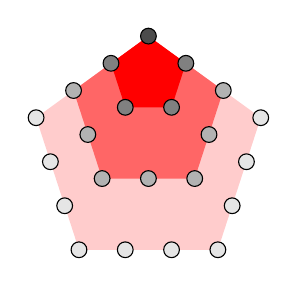
\begin{tikzpicture}[scale=0.5]
\fill[red!20!white] (0,1)--(3*0.951,-2+3*0.309)--(3*0.588,-2-3*0.809)--(-3*0.588,-2-3*0.809)--(-3*0.951,-2+3*0.309);
\fill[red!60!white] (0,1)--(2*0.951,-1+2*0.309)--(2*0.588,-1-2*0.809)--(-2*0.588,-1-2*0.809)--(-2*0.951,-1+2*0.309);
\fill[red] (0,1)--(0.951,0.309)--(0.588,-0.809)--(-0.588,-0.809)--(-0.951,0.309);

\fill[black!70!white] (0,1) circle(0.2 cm);
\fill[black!50!white] (0.951,0.309) circle(0.2 cm);
\fill[black!50!white] (-0.951,0.309) circle(0.2 cm);
\fill[black!50!white] (0.588,-0.809) circle(0.2 cm);
\fill[black!50!white] (-0.588,-0.809) circle(0.2 cm);

\draw (0,1) circle(0.2 cm);
\draw (0.951,0.309) circle(0.2 cm);
\draw (-0.951,0.309) circle(0.2 cm);
\draw (0.588,-0.809) circle(0.2 cm);
\draw (-0.588,-0.809) circle(0.2 cm);

\fill[black!30!white] (2*0.951,-1+2*0.309) circle(0.2 cm);
\fill[black!30!white] (1.539,-1.5) circle(0.2 cm);
\fill[black!30!white] (-2*0.951,-1+2*0.309) circle(0.2 cm);
\fill[black!30!white] (-1.539,-1.5) circle(0.2 cm);
\fill[black!30!white] (2*0.588,-1-2*0.809) circle(0.2 cm);
\fill[black!30!white] (-2*0.588,-1-2*0.809) circle(0.2 cm);
\fill[black!30!white] (0,-1-2*0.809) circle(0.2 cm);

\draw (2*0.951,-1+2*0.309) circle(0.2 cm);
\draw (1.539,-1.5) circle(0.2 cm);
\draw (-2*0.951,-1+2*0.309) circle(0.2 cm);
\draw (-1.539,-1.5) circle(0.2 cm);
\draw (2*0.588,-1-2*0.809) circle(0.2 cm);
\draw (-2*0.588,-1-2*0.809) circle(0.2 cm);
\draw (0,-1-2*0.809) circle(0.2 cm);

\fill[black!10!white] (3*0.951,-2+3*0.309) circle(0.2 cm);
\fill[black!10!white] (3*0.951-0.363,-2+3*0.309-1.118) circle(0.2 cm);
\fill[black!10!white] (3*0.951-2*0.363,-2+3*0.309-2*1.118) circle(0.2 cm);
\fill[black!10!white] (-3*0.951,-2+3*0.309) circle(0.2 cm);
\fill[black!10!white] (-3*0.951+0.363,-2+3*0.309-1.118) circle(0.2 cm);
\fill[black!10!white] (-3*0.951+2*0.363,-2+3*0.309-2*1.118) circle(0.2 cm);
\fill[black!10!white] (3*0.588,-2-3*0.809) circle(0.2 cm);
\fill[black!10!white] (-3*0.588,-2-3*0.809) circle(0.2 cm);
\fill[black!10!white] (-3*0.588+1.17557,-2-3*0.809) circle(0.2 cm);
\fill[black!10!white] (-3*0.588+2*1.17557,-2-3*0.809) circle(0.2 cm);

\draw (3*0.951,-2+3*0.309) circle(0.2 cm);
\draw (3*0.951-0.363,-2+3*0.309-1.118) circle(0.2 cm);
\draw (3*0.951-2*0.363,-2+3*0.309-2*1.118) circle(0.2 cm);
\draw (-3*0.951,-2+3*0.309) circle(0.2 cm);
\draw (-3*0.951+0.363,-2+3*0.309-1.118) circle(0.2 cm);
\draw (-3*0.951+2*0.363,-2+3*0.309-2*1.118) circle(0.2 cm);
\draw (3*0.588,-2-3*0.809) circle(0.2 cm);
\draw (-3*0.588,-2-3*0.809) circle(0.2 cm);
\draw (-3*0.588+1.17557,-2-3*0.809) circle(0.2 cm);
\draw (-3*0.588+2*1.17557,-2-3*0.809) circle(0.2 cm);
\end{tikzpicture}
\begin{tabular}{c|c|c|c|c|c|c|c}
$k$& -3&-2&-1&0&1&2&3\\
$\frac{3k^2-k}{2}$ & 15& 7& 2& 0& 1& 5& 12
\end{tabular}
\end{center}
\end{block}
}

\frame{\frametitle{Proof}

Consider a diagram of a partition of $n$ into different parts.\\
\begin{center}
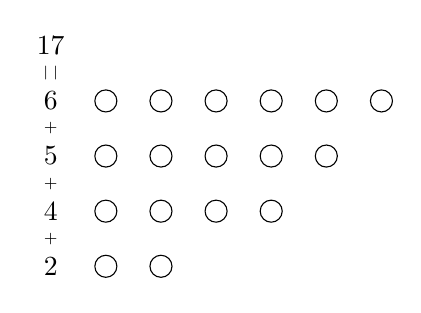
\begin{tikzpicture}[scale=0.7]
\draw (-1,1) node{$17$};
\draw (-1,0.5) node{$\scriptscriptstyle\mid\,\mid$};
\draw (-1,0) node{$6$};
\draw (-1,-0.5) node{$\scriptscriptstyle+$};
\draw (0,0) circle(0.2 cm);
\draw (1,0) circle(0.2 cm);
\draw (2,0) circle(0.2 cm);
\draw (3,0) circle(0.2 cm);
\draw (4,0) circle(0.2 cm);
\draw (5,0) circle(0.2 cm);
\draw (-1,-1) node{$5$};
\draw (-1,-1.5) node{$\scriptscriptstyle+$};
\draw (0,-1) circle(0.2 cm);
\draw (1,-1) circle(0.2 cm);
\draw (2,-1) circle(0.2 cm);
\draw (3,-1) circle(0.2 cm);
\draw (4,-1) circle(0.2 cm);
\draw (-1,-2) node{$4$};
\draw (-1,-2.5) node{$\scriptscriptstyle+$};
\draw (0,-2) circle(0.2 cm);
\draw (1,-2) circle(0.2 cm);
\draw (2,-2) circle(0.2 cm);
\draw (3,-2) circle(0.2 cm);
\draw (-1,-3) node{$2$};
\draw (0,-3) circle(0.2 cm);
\draw (1,-3) circle(0.2 cm);
\end{tikzpicture}
\end{center}
}



\frame{\frametitle{Proof}

Consider a diagram of a partition of $n$ into different parts.\\
\begin{center}
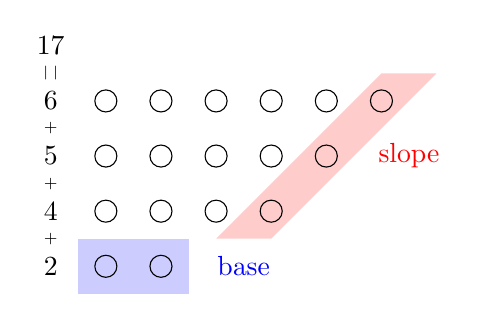
\begin{tikzpicture}[scale=0.7]
\fill[blue!20!white] (-0.5,-3.5)--(1.5,-3.5)--(1.5,-2.5)--(-0.5,-2.5);
\fill[red!20!white] (2.,-2.5)--(3.,-2.5)--(6.,0.5)--(5.,0.5);
\draw (5.5,-1) node{\color{red}slope};
\draw (2.5,-3) node{\color{blue}base};
\draw (-1,1) node{$17$};
\draw (-1,0.5) node{$\scriptscriptstyle\mid\,\mid$};
\draw (-1,0) node{$6$};
\draw (-1,-0.5) node{$\scriptscriptstyle+$};
\draw (0,0) circle(0.2 cm);
\draw (1,0) circle(0.2 cm);
\draw (2,0) circle(0.2 cm);
\draw (3,0) circle(0.2 cm);
\draw (4,0) circle(0.2 cm);
\draw (5,0) circle(0.2 cm);
\draw (-1,-1) node{$5$};
\draw (-1,-1.5) node{$\scriptscriptstyle+$};
\draw (0,-1) circle(0.2 cm);
\draw (1,-1) circle(0.2 cm);
\draw (2,-1) circle(0.2 cm);
\draw (3,-1) circle(0.2 cm);
\draw (4,-1) circle(0.2 cm);
\draw (-1,-2) node{$4$};
\draw (-1,-2.5) node{$\scriptscriptstyle+$};
\draw (0,-2) circle(0.2 cm);
\draw (1,-2) circle(0.2 cm);
\draw (2,-2) circle(0.2 cm);
\draw (3,-2) circle(0.2 cm);
\draw (-1,-3) node{$2$};
\draw (0,-3) circle(0.2 cm);
\draw (1,-3) circle(0.2 cm);
\end{tikzpicture}
\end{center}
}



\frame{
\begin{block}{}We define the following two operations on the diagrams and denote them $\alpha$ and $\beta$.
\end{block}

\begin{block}{$\mathbf{\alpha}$:} If $|b|\leq |s|$ and if $b$ and $s$ have no common point, or if $|b|\leq |s|-1$\\
Then we move $b$ up and turn its points into new slope.
\end{block}

\begin{block}{$\mathbf{\beta}$:} If $|b|> |s|$ and if $b$ and $s$ have no common point, or if $|b|\geq |s|+2$\\
Then we move the slope down and turn its points into the new base.
\end{block}

\begin{block}{}
\color{gray} If $b$ and $s$ have a common point and $|b|=|s|$ or $|b|=|s|+1$ then neither $\alpha$ no $\beta$ can be applied.
\end{block}

}

\frame{
\begin{block}{$\alpha$}
\begin{center}
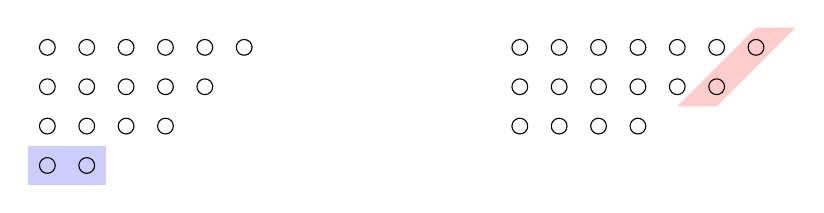
\begin{tikzpicture}[scale=0.5]

\fill[blue!20!white] (-0.5,-3.5)--(1.5,-3.5)--(1.5,-2.5)--(-0.5,-2.5);

\draw (0,0) circle(0.2 cm);
\draw (1,0) circle(0.2 cm);
\draw (2,0) circle(0.2 cm);
\draw (3,0) circle(0.2 cm);
\draw (4,0) circle(0.2 cm);
\draw (5,0) circle(0.2 cm);

\draw (0,-1) circle(0.2 cm);
\draw (1,-1) circle(0.2 cm);
\draw (2,-1) circle(0.2 cm);
\draw (3,-1) circle(0.2 cm);
\draw (4,-1) circle(0.2 cm);

\draw (0,-2) circle(0.2 cm);
\draw (1,-2) circle(0.2 cm);
\draw (2,-2) circle(0.2 cm);
\draw (3,-2) circle(0.2 cm);

\draw (0,-3) circle(0.2 cm);
\draw (1,-3) circle(0.2 cm);



\begin{scope}[xshift=12 cm]

\fill[red!20!white] (4.,-1.5)--(5.,-1.5)--(7.,0.5)--(6.,0.5);

\draw (0,0) circle(0.2 cm);
\draw (1,0) circle(0.2 cm);
\draw (2,0) circle(0.2 cm);
\draw (3,0) circle(0.2 cm);
\draw (4,0) circle(0.2 cm);
\draw (5,0) circle(0.2 cm);
\draw (6,0) circle(0.2 cm);

\draw (0,-1) circle(0.2 cm);
\draw (1,-1) circle(0.2 cm);
\draw (2,-1) circle(0.2 cm);
\draw (3,-1) circle(0.2 cm);
\draw (4,-1) circle(0.2 cm);
\draw (5,-1) circle(0.2 cm);

\draw (0,-2) circle(0.2 cm);
\draw (1,-2) circle(0.2 cm);
\draw (2,-2) circle(0.2 cm);
\draw (3,-2) circle(0.2 cm);
\end{scope}
\end{tikzpicture}
\end{center}
\end{block}


\begin{block}{$\beta$}
\begin{center}
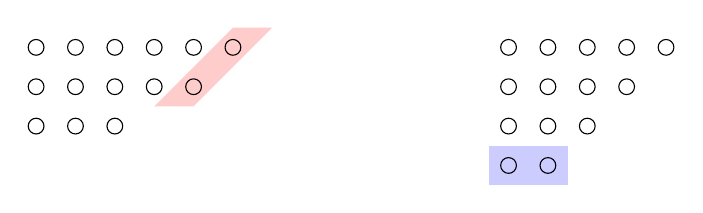
\begin{tikzpicture}[scale=0.5]

\fill[red!20!white] (3.,-1.5)--(4.,-1.5)--(6.,0.5)--(5.,0.5);

\draw (0,0) circle(0.2 cm);
\draw (1,0) circle(0.2 cm);
\draw (2,0) circle(0.2 cm);
\draw (3,0) circle(0.2 cm);
\draw (4,0) circle(0.2 cm);
\draw (5,0) circle(0.2 cm);

\draw (0,-1) circle(0.2 cm);
\draw (1,-1) circle(0.2 cm);
\draw (2,-1) circle(0.2 cm);
\draw (3,-1) circle(0.2 cm);
\draw (4,-1) circle(0.2 cm);

\draw (0,-2) circle(0.2 cm);
\draw (1,-2) circle(0.2 cm);
\draw (2,-2) circle(0.2 cm);


\begin{scope}[xshift=12 cm]

\fill[blue!20!white] (-0.5,-3.5)--(1.5,-3.5)--(1.5,-2.5)--(-0.5,-2.5);

\draw (0,0) circle(0.2 cm);
\draw (1,0) circle(0.2 cm);
\draw (2,0) circle(0.2 cm);
\draw (3,0) circle(0.2 cm);
\draw (4,0) circle(0.2 cm);


\draw (0,-1) circle(0.2 cm);
\draw (1,-1) circle(0.2 cm);
\draw (2,-1) circle(0.2 cm);
\draw (3,-1) circle(0.2 cm);


\draw (0,-2) circle(0.2 cm);
\draw (1,-2) circle(0.2 cm);
\draw (2,-2) circle(0.2 cm);

\draw (0,-3) circle(0.2 cm);
\draw (1,-3) circle(0.2 cm);
\end{scope}
\end{tikzpicture}
\end{center}
\end{block}
}

\frame{
\begin{block}{}
To each diagram $D$ we can apply at most one of the operations $\alpha$ or $\beta$.
\end{block}
\begin{block}{}
If $\alpha$ can be applied to $D$ then $\beta$ can be applied to $\alpha(D)$.
\end{block}
\begin{block}{}
If $\beta$ can be applied to $D$ then $\alpha$ can be applied to $\beta(D)$.
\end{block}
}

\frame{
\begin{block}{}Thus we have a 1:1 correspondence
\end{block}
\begin{block}{}
$$\left\{\begin{smallmatrix}
          \mbox{odd partitions}\\
          \mbox{into distinct parts} \\
          \mbox{s. t. }\alpha\mbox{ or }\beta\mbox{ can be applied }
        \end{smallmatrix}\right\}\leftrightarrow
\left\{\begin{smallmatrix}
          \mbox{even partitions}\\
          \mbox{into distinct parts} \\
          \mbox{s. t. }\alpha\mbox{ or }\beta\mbox{ can be applied }
        \end{smallmatrix}\right\}$$
\end{block}

}

\frame{
\begin{block}{}When can neither $\alpha$ nor $\beta$ be applied?
\begin{itemize}
\item $b$ and $s$ have a common point and $|b|=|s|=k$
$$n=k+(k+1)+\ldots+(2k-1)=\frac{3k^2-k}{2}.$$
\item  $b$ and $s$ have a common point and $|b|-1=|s|=k$
$$n=(k+1)+\ldots+2k=\frac{3k^2+k}{2}.$$
\end{itemize}
\end{block}

\begin{block}{}Therefore:
$$p_e(n)-p_o(n)=c_n=
\begin{cases}(-1)^k,&\mbox{ if } n= \frac{3k^2\pm k}{2}\\
0, & \mbox{otherwise.}\end{cases}$$

This finishes the proof.
\end{block}
}

\frame{\frametitle{Jacobi triple product}
\begin{block}{Theorem}
For all $w\neq 0$ and $q$ with $|q|<1$:
$$\prod_{k=1}^\infty (1-q^{2k})\,(1-q^{2k-1}\,w^2)\,(1-q^{2k-1}\,w^{-2})=\sum_{k=-\infty}^\infty (-1)^k\,w^{2k}\,q^{k^2}.$$
\end{block}
}

\frame{\frametitle{Proof}
Set
$
\phi_n(w,q):=\prod_{k=1}^n(1-q^{2k-1}\,w^2)\,(1-q^{2k-1}\,w^{-2}).
$
We have
\begin{equation}\label{eqn: 1}\phi_n(qw,q)\,=\,\phi_n(w,q)\,\frac{(1-q^{2n+1}\,w^2)\,(1-q^{-1}w^{-2})}
{(1-qw^2)\,(1-q^{2n-1}w^{-2})}\,=\,\phi_n(w,q)\,\frac{1-q^{2n+1}\,w^2}{-qw^2+q^{2n}}.
\end{equation}
We consider the following expansion
\begin{equation}\label{eqn: 2}
\phi_n(w,q)=\sum_{k=-n}^nA_{n,k}(q)\,w^{2k},
\end{equation}
where $A_{n,k}(q)$ is a polynomial in $q$. We have a symmetry $A_{n,k}(q)=A_{n,-k}(q)$.
We find
\begin{equation}\label{eqn: 3}
A_{n,n}(q)=q^{1+3+5+\ldots+(2n-1)}=q^{n^2}.
\end{equation}
We substitute \eqref{eqn: 2} into \eqref{eqn: 1} and obtain
\begin{equation}\label{eqn: 4}
A_{n,k}(q)=A_{n,k-1}(q)\,q^{2k-1}\,\frac{1-q^{2n-2k+2}}{1-q^{2n+2k}}.
\end{equation}
}

\frame{
From \eqref{eqn: 3} and \eqref{eqn: 4} we find
\begin{equation}\label{eqn: 5}
A_{n,k}=\frac{q^{k^2}}{(1-q^2)\cdots(1-q^{2n})}\,\prod_{s=n-k+1}^n(1-q^{2s})\,\prod_{s=n+k+1}^{2n}(1-q^{2s}).
\end{equation}
From \eqref{eqn: 5} we obtain
$$\prod_{k=1}^n (1-q^{2k})\,(1-q^{2k-1}\,w^2)\,(1-q^{2k-1}\,w^{-2})=\sum_{k=-n}^n(-1)^k w^{2k}\,q^{k^2}\,B_{n,k}(q).$$
where
$$B_{n,k}(q)=\prod_{s=n-k+1}^n(1-q^{2s})\,\prod_{s=n+k+1}^{2n}(1-q^{2s}).$$
We have $B_{n,k}=1+O(q^{n-k+1})$.
We take the limit $n\to \infty$ and  finish the proof.
}






















\end{document}
